\documentclass[mathserif]{beamer}
\usetheme[secheader]{pecostalk}
\graphicspath{{figs/}}                                                                                                                              

%\usepackage{verbatim}
\usepackage{tikz}

\newcommand{\red}[1]{{\color{red}#1}}

\newcommand{\UQ}[1]{{\color{red}{#1}}}

\newcommand{\abs}[1]{\ensuremath{ \left|#1\right|}}
\newcommand{\norm}[1]{\ensuremath{ \left|\left|#1\right|\right|}}
\newcommand{\orderof}[1]{\ensuremath{ {\cal O}\left(#1\right)}}
\newcommand{\pdv}[2]{\frac{\partial #1}{\partial #2}}
\newcommand{\grad}[1]{\bv{\nabla} {#1}}
\newcommand{\bv}[1]{{\ensuremath{\boldsymbol{#1}}}}
\newcommand{\bt}[1]{{\ensuremath{\boldsymbol{#1}}}}

\newcommand{\Res}{{\ensuremath{\mathcal R}}}
\newcommand{\Unknowns}{{\ensuremath{\bf{U}}}}
\newcommand{\UnknownsR}{{\ensuremath{\bf{U^R}}}}
\newcommand{\unknown}{{\ensuremath{\bv{u}}}}
\newcommand{\primalsol}{{\ensuremath{\bv{\tilde{u}}}}}
\newcommand{\primalsolh}{{\ensuremath{\bv{\tilde{u}^h}}}}
\newcommand{\adjointsol}{{\ensuremath{\bv{\tilde{z}}}}}
\newcommand{\adjointsolh}{{\ensuremath{\bv{\tilde{z}^h}}}}
\newcommand{\adjointsolH}{{\ensuremath{\bv{\tilde{z}^H}}}}
\newcommand{\Testfuncs}{{\ensuremath{\bf{V}}}}
\newcommand{\testfunc}{{\ensuremath{\bv{v}}}}

\newcommand{\intO}{\ensuremath{\int_\Omega}}
\newcommand{\elem}{\ensuremath{E}}
\newcommand{\qoi}{{\ensuremath{q}}}
\newcommand{\qoih}{\ensuremath{q^h}}
\newcommand{\Qoi}{{\ensuremath{Q}}}
\newcommand{\param}{{\ensuremath{\xi}}}
\newcommand{\params}{{\ensuremath{\bv{\param}}}}
\newcommand{\PDF}{\ensuremath{p}}
\newcommand{\Params}{{\ensuremath{\bf{\Xi}}}}
\newcommand{\ParamsR}{{\ensuremath{\bf{\Xi^R}}}}

\newcommand{\Reals}{{\ensuremath{\mathbb{R}}}}


\newcommand{\sa}{\nu_{\mathrm{sa}}}
\newcommand{\pp}[2]{\frac{\partial #1}{\partial #2}}

\newcommand{\software}[1]{\texttt{#1}}
\newcommand{\code}[1]{\software{#1}}
\newcommand{\GRINS}{\software{GRINS}}
\newcommand{\libMesh}{\software{libMesh}}

\definecolor{DarkGreen}{rgb}{0.13,0.55,0.13}
\definecolor{DarkRed}{rgb}{0.55,0.13,0.13}
%\newcommand{\CVer}[1]{{\color{DarkGreen}{#1}}}
\newcommand{\CVer}[1]{#1}
%\newcommand{\CVal}[1]{{\color{blue}{#1}}}
\newcommand{\CVal}[1]{#1}
%\newcommand{\CUQ}[1]{{\color{purple}{#1}}}
\newcommand{\CUQ}[1]{#1}
%\newcommand{\CInt}[1]{{\color{orange}{#1}}}
\newcommand{\CInt}[1]{#1}
%\newcommand{\CExa}[1]{{\color{brown}{#1}}}
\newcommand{\CExa}[1]{#1}

\date{January 14, 2013}
\author[R. H. Stogner]{Roy H. Stogner}
\institute{The University of Texas at Austin}
\title[\libMesh]{Integrated Simulation Software:\\
\libMesh{} Finite Element Library}
%\libMesh: Tools for Parallel Computation on Adaptive Discretizations}

\begin{document}
\begin{frame}
\begin{center}
\includegraphics[width=.8\linewidth]{grand_logo}\\
\end{center}
\titlepage
\vspace{-0.4in}
\includegraphics[width=0.15\linewidth]{ICES-secondary-logo-crop}
\hspace*{\fill}
\includegraphics[scale=0.2]{asc_logo}
\end{frame}



%===============================================================================
\section{Motivation}


%===============================================================================
\begin{frame}
\frametitle{Motivation: Predictive Simulation Requirements}
\begin{block}{\CVer{Verified}, \CVal{Validated}, \CInt{Integrated
Multidisciplinary} Simulations with \CUQ{Uncertainty
Quantification} at \CExa{Exascale}}
\begin{itemize}
\item \CInt{New model requirements} arise from \CUQ{sensitivity studies}
\item All physics coded for full system uncertainty propagation should
\CExa{be massively parallel} and \CExa{system independent}
\item Rapid \CVer{code verification}, \CVal{model validation} needed
for each physics
\item \CInt{Multiphysics model coupling} code may require \CVer{joint testing}
\item \CVer{Estimation of discretization error and model error}
is part of every \CUQ{uncertainty problem}
\end{itemize}
\end{block}
\end{frame}


%===============================================================================
\begin{frame}
\frametitle{Software Design Principles}
\begin{block}{Design Separation}
Interfaces must expose complex functionality but still enable
independent implementation development for:
\begin{itemize}
\item \CExa{Numerics optimization}: discretization vs. algebraic solver code
\item \CExa{Code optimization}: physics vs. system assembly code
\item \CVer{Code verification}: module uses vs. unit tests
\item \CVer{Solution verification}: physics vs. error estimation code
\item \CUQ{Uncertainty quantification}: simulation vs. UQ code
\item \CInt{Interdisciplinary collaboration}: physics vs. any code
\end{itemize}
\end{block}

The \libMesh{} Finite Element Method (FEM) library provides:
\begin{itemize}
	\item Application Programming Interfaces (APIs) for such designs
	\item Implementations of physics-independent FEM code
	\item Common interfaces to third-party tools
\end{itemize}

\end{frame}



%===============================================================================
\section{Verification}


%===============================================================================
\begin{frame}
\frametitle{Verification: Code Verification}

\begin{columns}
\column{.45\textwidth}
\begin{block}{Component Tests}
\begin{itemize}
\item $\sim 6000$ internal assertions
\item $\sim 50$ example applications 
\item $\sim 120$ unit tests
\item Continuous Integration (CI): all tests, $\sim 12$ configurations
\end{itemize}
\end{block}

\column{.45\textwidth}
\begin{block}{Application Tests}
\begin{itemize}
\item \texttt{FIN-S}, \texttt{GRINS}, \texttt{MOOSE}
\item Unit, regression, full tests with detailed physics
\item MMS solution verification via {\texttt{MASA}} library
\item Buildbot, Trac CI
\end{itemize}
\end{block}
\end{columns}

\begin{columns}
\column{.55\textwidth}
\begin{block}{Method of Manufactured Solutions (MMS)}
\begin{itemize}
	\item $F(u) = 0$ (analytic strong PDE)
	\item $\hat{F}(v) \equiv F(v) - F(\hat{u})$ ({\texttt{MASA}})
	\item $\hat{F}(u_h) \rightarrow 0$ (Application)
	\item $\norm{\hat{u} - \hat{u_h}} < C N^r$ (Verification)
\end{itemize}
\end{block}

\column{.45\textwidth}
\center
\includegraphics[width=.8\textwidth]{mms_grid_convergence}

\end{columns}

\end{frame}

%===============================================================================
\begin{frame}
\frametitle{Solution Verification}
\begin{block}{\emph{A Posteriori} Error Estimation}
\begin{itemize}
	\item Global estimates
	\begin{itemize}
		\item Refinement, residual: approximation error
			$\norm{u-u_h}_\mathcal{H} \approx
			\norm{u_H-u_h}_\mathcal{H}$
		\begin{itemize}
			\item residual-based: physics-specific!
		\end{itemize}
		\item Patch recovery: interpolation error
			$\norm{u-u_h}_\mathcal{H} \approx
			C \norm{u-\Pi u}_\mathcal{H}$
		\begin{itemize}
			\item Calibrate approximation bound $C$ via \texttt{MASA}?
		\end{itemize}
	\end{itemize}
	\item Quantity of interest error estimates
	\begin{itemize}
		\item Refinement-based: $\Qoi(u) - \Qoi(u_h) \approx
			\Qoi(u_H) - \Qoi(u_h)$
		\item Adjoint-based: $\Qoi(u) - \Qoi(u_h) \approx \Res(-u_h, z)$
	\end{itemize}
	\end{itemize}
\end{block}


\end{frame}



%===============================================================================
\section{Adaptivity}


%===============================================================================
\begin{frame}
\frametitle{Adaptivity: Error Estimators, Error Indicators}
\begin{columns}
\column{.7\textwidth}
\begin{block}{Error decompositions}
	Subterms on each element $K$:
	\begin{itemize}
		\item $\norm{u-u_h}_\mathcal{H}^2 = 
			\sum_K \norm{u-u_h}_\mathcal{H(K)}^2 \leq 
			\sum_K \abs{\eta_K}^2$
		\item $\Qoi(u) - \Qoi(u_h) \approx \sum_K \eta_K$
		\item $\abs{\Qoi(u) - \Qoi(u_h)} \leq \sum_K \abs{\eta_K}$
	\end{itemize}
\end{block}
\begin{block}{Refinement heuristics}
	\begin{itemize}
	\item Refinement/coarsening of elements with:
	\begin{itemize}
		\item Worst/best fraction sorted by error
		\item Error over/under fraction of tolerance
		\item Error over/under target mesh size average
	\end{itemize}
	\item $h$-vs-$p$ refinement:
	\begin{itemize}
		\item {\textit{a priori}} singularity identification
		\item Behavior vs. cost when $h$ vs. $p$ coarsening?
	\end{itemize}
	\end{itemize}
\end{block}

\column{.3\textwidth}
\center
\includegraphics[width=.6\textwidth]{qoi_primal_error}

\center
\includegraphics[width=.6\textwidth]{qoi_weighted_error}
\end{columns}
\end{frame}


%===============================================================================
\begin{frame}
\frametitle{Adaptive Mesh Refinement}

\begin{block}{Refinement types}
\begin{columns}
\column{.65\textwidth}
\begin{itemize}
\item In \libMesh{} code:
\begin{itemize}
\item Isotropic hanging-node $h$-refinement
\item Hierarchic $p$-refinement
\item Mesh redistribution
\end{itemize}
\item \libMesh{} compatible:
\begin{itemize}
\item Simplex edge splitting
\item Weighted mesh regeneration
\end{itemize}
\end{itemize}
\column{.35\textwidth}
\center
\includegraphics[width=.25\textwidth]{adaptive}

\center
\includegraphics[width=.8\textwidth]{PHierarchic}
\end{columns}
\end{block}

\begin{block}{Refinement Utilities}
\begin{itemize}
\item Projection-based interpolation
\begin{itemize}
\item $\orderof{N_e}$ on nested meshes
\item $\orderof{N_e \log{N_e}}$ on arbitrary meshes
\end{itemize}
\item Projection from functors for Initial Conditions (IC)
\item {\texttt{ExactErrorEstimator}} for IC mesh refinement
\end{itemize}
\end{block}

\end{frame}


%===============================================================================
\begin{frame}
\frametitle{Goal-oriented Adaptivity}

\begin{columns}

\column{0.5\textwidth}
Refine to reduce solution error {\emph{when it influences QoI error}}:

\begin{center}
\includegraphics[width=1.0\textwidth]{qoi_may_29_2009_convergence_cropped}
\end{center}

\column{0.45\textwidth}

\begin{center}
\includegraphics[height=0.5\textwidth]{QoI_October_20_2011_kelly_mesh}
\includegraphics[height=0.5\textwidth]{QoI_May_29_2009_arpp_mesh+adjoint}
\end{center}

\begin{itemize}
\item Global error indicator ignores QoI sensitivity, plateaus
\item Rapid convergence from adjoint-based refinement
\end{itemize}

\end{columns}

\end{frame}


%===============================================================================
\begin{frame}
\frametitle{Adjoint-based Goal-oriented Error Indicators}

\begin{equation*}
\Qoi(\primalsolh) - \Qoi(\primalsol) = \Res(\primalsolh, \adjointsol; \params) + H.O.T.
\end{equation*}

\begin{block}{Adjoint Refinement}
\begin{equation*}
\Res(\primalsolh, \adjointsol; \params) = \sum_\elem 
\Res^\elem(\primalsolh, \adjointsolH; \params)
\end{equation*}
\end{block}

\begin{block}{Adjoint Residual}
\begin{equation*}
\abs{\Res(\primalsolh, \adjointsol; \params)} \leq
\sum_\elem \norm{\Res^\elem_\unknown}_{B(\Unknowns^\elem,
\Testfuncs^{\elem *})}
\norm{\primalsol - \primalsolh}_{\Unknowns^\elem}
\norm{\adjointsol - \adjointsolh}_{\Testfuncs^\elem}
\end{equation*}
\end{block}

\begin{block}{Generalized Adjoint Residual}
\begin{align*}
\abs{\Res(\primalsolh, \adjointsol; \params)}
\leq \sum_\elem \norm{\adjointsol_i-\adjointsolh_i}_i \; M_{ij} \; \norm{\primalsol_j-\primalsolh_j
}_j \nonumber
\end{align*}
\end{block}

\end{frame}



%===============================================================================
\section{Uncertainty Quantification}


%===============================================================================
\begin{frame}
\frametitle{UQ: Adjoint-based Sensitivities, Surrogates}

\begin{equation*}
\frac{d \qoi}{d \params} = \Qoi_\params(\primalsol; \params) -
 \Res_\params(\primalsol, \adjointsol; \params)
\end{equation*}

\begin{itemize}
\item Uses same linear adjoint solution as equal-order estimators
\item One linear solve per QoI, one residual evaluation per parameter
\item Automatic adjoint-of-discretization {\texttt{adjoint\_solve()}}
\item Transient adjoint support being added to \libMesh
\end{itemize}

\begin{block}{Certified Reduced Basis Models}
\begin{itemize}
	\item Low-order problems for accurate QoI data on linear(ized) PDEs
\end{itemize}
\end{block}

\begin{block}{Response Surface Interpolants}
\begin{itemize}
	\item Local Sensitivity Derivative Enhanced Monte Carlo
%		$\hat{\primalsol}(\params) \equiv
%		\primalsol_n + \nabla \primalsol_n
%		\left(\params - \params_n\right)$
	\item Gradient+value interpolants
\end{itemize}
\end{block}

\end{frame}



%===============================================================================
\section{Scalability}


%===============================================================================
\begin{frame}
\frametitle{Scalability: Hybrid MPI + Threads}

\begin{columns}
\column{.65\textwidth}
\begin{block}{Parallel:: interfaces wrap MPI}
Library data is distributed, synchronized:
\begin{itemize}
	\item Simpler, STL-compatible, inlined API
	\item Works with complex serializable classes
\end{itemize}
\end{block}

\begin{block}{Threads:: interfaces wrap TBB}
Many library functions are multi-threaded:
\begin{itemize}
	\item Sparsity, AMR constraint calculation
	\item {\texttt{FEMSystem}} assembly routines
	\item Asynchronous I/O
	\item Mesh projections, utility functions
\end{itemize}
\end{block}

\column{.35\textwidth}
\center
\includegraphics[width=.8\textwidth]{fins_speedup}

\center
\includegraphics[width=.8\textwidth]{threaded_speedup}

\end{columns}

\begin{itemize}
	\item Hybrid parallel apps with {\emph{no}}
		threading or message passing code
	\item API-independence via \libMesh{} wrappers
\end{itemize}
\end{frame}


%===============================================================================
\begin{frame}
\frametitle{Shared- vs. Distributed-Memory Mesh Parallelism}
\begin{columns}
\column{.6\textwidth}
\begin{block}{Distributed Storage}
	\begin{itemize}
		\item Each rank owns ``local'' elements
		\item Copies ``semilocal'' node-neighbors
	\end{itemize}
\end{block}
\begin{block}{Distributed Operations}
	\begin{itemize}
		\item Two-pass DoF numbering
		\item Recursive constraint push/pull
		\item Sparsity data synchronization
		\item AMR flag condition satisfaction
		\item AMR element creation
		\item Repartitioning, redistribution
	\end{itemize}
\end{block}
\column{.4\textwidth}
\center
\includegraphics[width=.7\textwidth]{SerialMesh}

\center
\includegraphics[width=.7\textwidth]{ParallelMesh1}
\end{columns}
\end{frame}



%===============================================================================
\section{Future Plans}


%===============================================================================
\begin{frame}
\frametitle{Future Plans: Hybrid MPI + Threads + Accelerators}

\begin{columns}
\column{.4\textwidth}
\includegraphics[width=\textwidth]{DofObjects}

\vspace{.1\textwidth}

\includegraphics[width=\textwidth]{FEMSystem}

\column{.6\textwidth}
\begin{block}{API Levels}
\begin{enumerate}
	\item Basic \libMesh{} objects, iterators
	\begin{itemize}
		\item Greatest flexibility
		\item Easy message-passing parallelism
		\item Automatic steady near-adjoints
	\end{itemize}
	\item {\texttt{FEMSystem}} framework 
	\begin{itemize}
		\item More structured design
		\item Automatic multithreaded assembly
		\item Automatic exact, transient adjoints
		\item Intrusive UQ assembly?
	\end{itemize}
	\item {\texttt{MetaPhysics}} functors
	\begin{itemize}
		\item \libMesh{} independence
		\item Compile-time physics composition
		\begin{itemize}
			\item Run-time optional?
		\end{itemize}
		\item Automatic GPGPU use via \texttt{Thrust}?
		\item \LaTeX{} OO, other specialized inputs?
	\end{itemize}
\end{enumerate}
\end{block}
\end{columns}
\end{frame}



%===============================================================================
\begin{frame}
\frametitle{Application Programming, Metaprogramming Interfaces}
\begin{columns}

\column{.6\textwidth}

\begin{block}{Current Metaprogramming Experiments}
\begin{itemize}
	\item {\texttt{CompileTimeContainer}} Meta-class with
		utilities for metaprogramming
	\item {\texttt{DualNumber}}, {\texttt{NumberArray}}
		$\rightarrow$ {\texttt{SparseNumberStruct}} nestable
		template classes for Automatic Differentiation
	\begin{itemize}
		\item Released as part of {\texttt{MASA}} for MMS construction
	\end{itemize}
	\item {\texttt{Equations}} container with compile-time
		physics-evaluation methods
	\begin{itemize}
		\item Submodel-independent code
		\item Physics dependency resolution
		\item Jacobian evaluation optimization?
		\item \texttt{Thrust} GPGPU compatibility?
	\end{itemize}
\end{itemize}
\end{block}

\column{.4\textwidth}
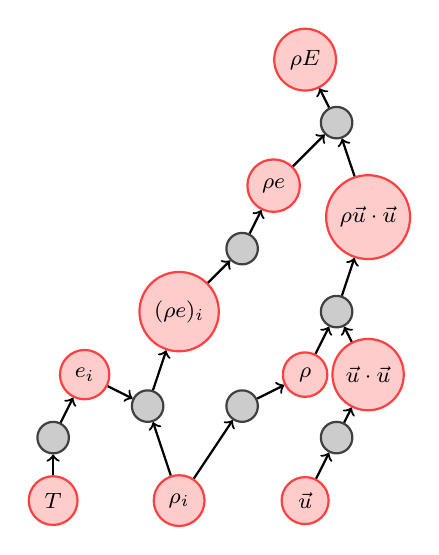
\begin{tikzpicture}[scale=.4]
	\tikzstyle{data}=[circle,thick,draw=red!75,fill=red!20,minimum size=3mm,font=\footnotesize]
	\tikzstyle{eqn}=[circle,thick,draw=black!75,fill=black!20,minimum size=4mm]

	\node [data] (T) at (0,0) {$T$};
	\node [data] (e_i) at (1,4) {$e_i$};
	\node [data] (rho_i) at (4,0) {$\rho_i$};
	\node [data] (rho_e_i) at (4,6) {$(\rho e)_i$};
	\node [data] (rho_e) at (7,10) {$\rho e$};
	\node [data] (rho) at (8,4) {$\rho$};
	\node [data] (u) at (8,0) {$\vec{u}$};
	\node [data] (u_sq) at (10,4) {$\vec{u}\cdot\vec{u}$};
	\node [data] (rho_u_sq) at (10,9) {$\rho \vec{u}\cdot\vec{u}$};
	\node [data] (rho_E) at (8,14) {$\rho E$};

	\node [eqn] (to_e_i) at (0,2) {};
	\node [eqn] (to_rho_e_i) at (3,3) {};
	\node [eqn] (to_rho_e) at (6,8) {};
	\node [eqn] (to_rho) at (6,3) {};
	\node [eqn] (to_u_sq) at (9,2) {};
	\node [eqn] (to_rho_u_sq) at (9,6) {};
	\node [eqn] (to_rho_E) at (9,12) {};

	\foreach \source/\dest in
	{T/to_e_i,rho_i/to_rho_e_i,e_i/to_rho_e_i,rho_e_i/to_rho_e,rho_i/to_rho,u/to_u_sq,rho/to_rho_u_sq,u_sq/to_rho_u_sq,rho_e/to_rho_E,rho_u_sq/to_rho_E}
	  \draw [->,thick](\source) to (\dest);

	  \foreach \source/\dest in
	  {to_e_i/e_i,to_rho_e_i/rho_e_i,to_rho_e/rho_e,to_rho/rho,to_u_sq/u_sq,to_rho_u_sq/rho_u_sq,to_rho_E/rho_E}
	    \draw [->,thick](\source) to (\dest);
\end{tikzpicture}

\end{columns}
\end{frame}


%===============================================================================
\section{\libMesh{} Usage}

%===============================================================================
\begin{frame}
\frametitle{\libMesh{} Usage: Publications}

\begin{block}{Ph.D. Theses}
\begin{itemize}
\item {\textbf{University of Texas:}} B.S.~Kirk, J.W.~Peterson, R.H.~Stogner,
	A.J.~Hawkins-Daarud, V.V.~Garg

\item {\textbf{University of Oxford:}} D.~Knezevic

\item {\textbf{Università Degli Studi Di Roma:}} E.~Petrolati

\item {\textbf{Graz University of Technology:}} M.~Nenning, L.~Nagler

\item {\textbf{ETH Z\"{u}rich:}} J.A.~Kallen-Brown

\item {\textbf{Massachusetts Institute of Technology:}} K.~Lee

\item {\textbf{Università di Bologna:}} G.~Bornia

\item {\textbf{COPPE/UFRJ:}} A.L.~Rossa
\end{itemize}
\end{block}

\begin{block}{Publications}
\begin{itemize}
\item ~150 peer-reviewed papers using and citing \libMesh{}
\item ~300 unique co-authors
\end{itemize}
\end{block}

\end{frame}


%===============================================================================
\begin{frame}
\frametitle{Current Developers, Acknowledgements}

\begin{columns}

\column{.45\textwidth}

\begin{block}{UT Austin - PECOS}
\begin{itemize}
\item Paul Bauman
\begin{itemize}
\item Vector-valued Elements
\end{itemize}
\item Roy Stogner
\begin{itemize}
\item Chief Software Architect
\end{itemize}
\end{itemize}
\includegraphics[width=\textwidth]{ablating_hs_wbg}
\end{block}

\column{.45\textwidth}
\begin{block}{NASA Johnson Space Center}
\begin{itemize}
\item Benjamin Kirk
\begin{itemize}
\item Creator, Manager
\end{itemize}
\end{itemize}
\includegraphics[width=\textwidth]{arcjet_ben_T}
\end{block}

\begin{block}{MIT - Aero. Astro., Mech. Eng.}
\begin{itemize}
\item Vikram Garg
\begin{itemize}
\item Adjoint Methods
\end{itemize}
\item Sylvain Vallaghe
\end{itemize}
\end{block}

\end{columns}

\end{frame}


%===============================================================================
\begin{frame}
\frametitle{Current Developers, Acknowledgements}
\begin{columns}
\column{.45\textwidth}

\begin{block}{Idaho National Laboratory}
\begin{itemize}
\item David Andrs
\item Derek Gaston
\item Cody Permann
\item John Peterson 
\end{itemize}
\center
\includegraphics[width=.8\textwidth]{moose}
\end{block}

\column{.45\textwidth}

\begin{block}{Argonne National Laboratory}
\begin{itemize}
\item Dmitry Karpeev 
\begin{itemize}
\item Advanced \texttt{PETSc} Functionality
\end{itemize}
\end{itemize}
\end{block}

\begin{block}{Akselos}
\begin{itemize}
\item David Knezevic
\begin{itemize}
\item Reduced Basis Methods
\end{itemize}
\end{itemize}
\center
\includegraphics[width=.8\textwidth]{mufflers_new}
\end{block}

\end{columns}
\end{frame}


%===============================================================================
% NEW SLIDE
%===============================================================================
%\begin{frame}
%\frametitle{}
%\begin{block}{}
%\center{Thank you!} \\
%\center{Questions?}
%\end{block}
%\end{frame}

 
\end{document}
%===============================================================================
% END OF FILE
%===============================================================================
